\documentclass{beamer}

\usepackage[utf8]{inputenc}
\usepackage{hyperref}

\usetheme{Berkeley}
\beamertemplatenavigationsymbolsempty
\setbeamertemplate{headline}{}
 
\title{Importing data into FoodChain-Lab 1}
\date{}
 
\begin{document}
\maketitle

\section{ }

\subsection{Tasks}
\begin{frame}
	\begin{itemize}
		\item In this tutorial we'll show you how to import delivery data to FoodChain-Lab via our Excel templates.
		\item We will first import the initial data for the outbreak locations and then successively add the delivery data for caterers and other suppliers via autogenerated back- and forward-tracing templates.
		\item In FoodChain-Lab it is also possible to import the whole delivery network from one Excel file, but that procedure is not documented here as it is advantageous. The underlying "All In One" template can be downloaded from here: \url{https://github.com/SiLeBAT/BfROpenLabResources/raw/master/GitHubPages/templates/All_In_One_Template.xlsx}.
	\end{itemize}
\end{frame}
 
\subsection{1}
\begin{frame}
	\begin{center}
  		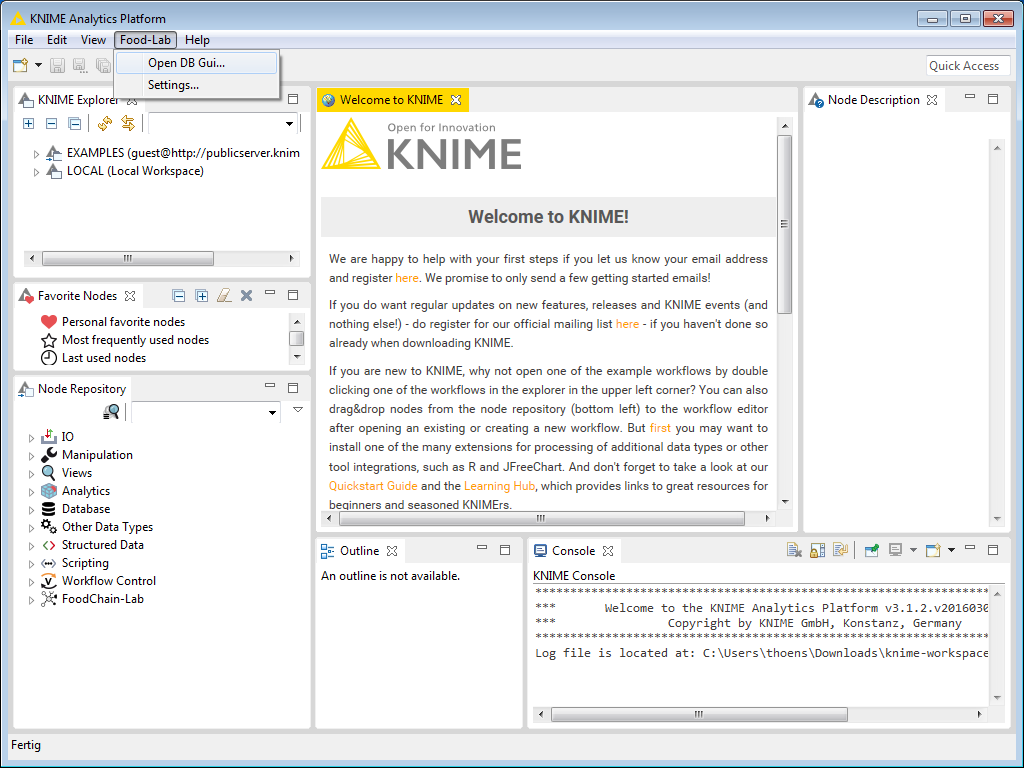
\includegraphics[height=0.6\textheight]{1.png}
	\end{center}
	\begin{itemize}
		\item Select \textbf{Food-Lab $>$ Open DB Gui...} in the menu bar to open the database interface.
	\end{itemize}
\end{frame}

\subsection{2}
\begin{frame}
	\begin{center}
  		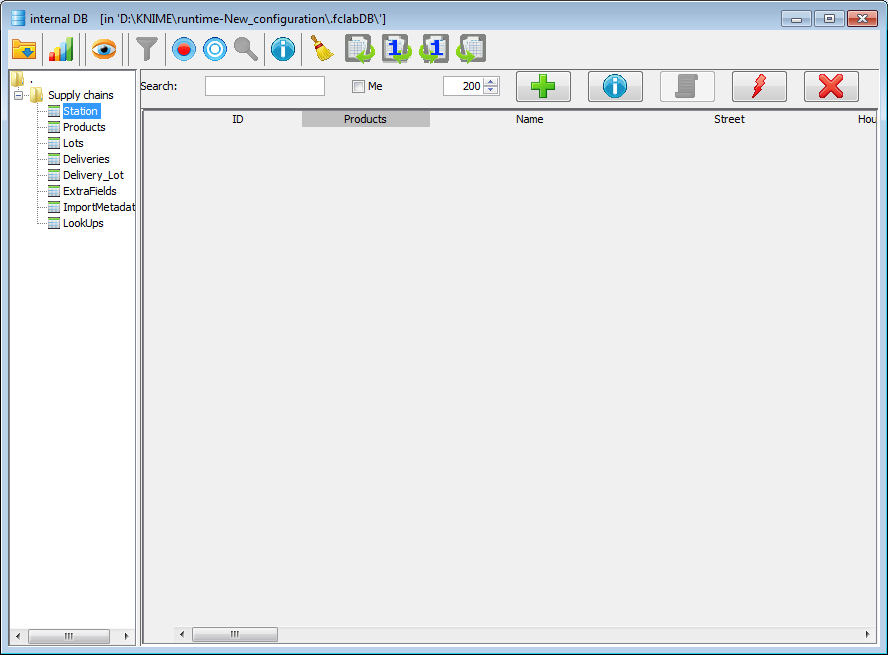
\includegraphics[height=0.5\textheight]{2.png}
	\end{center}
	\begin{itemize}
		\item The FoodChain-Lab database interface now pops up.
		\item Here you can import, edit and validate food delivery data.
		\item To start the data import you must download, fill out and import the "Start Tracing Template".
		\item It can be downloaded from here: \url{https://github.com/SiLeBAT/BfROpenLabResources/raw/master/GitHubPages/templates/Start_Tracing_Template.xlsx}.
	\end{itemize}
\end{frame}

\subsection{3}
\begin{frame}
	\begin{center}
  		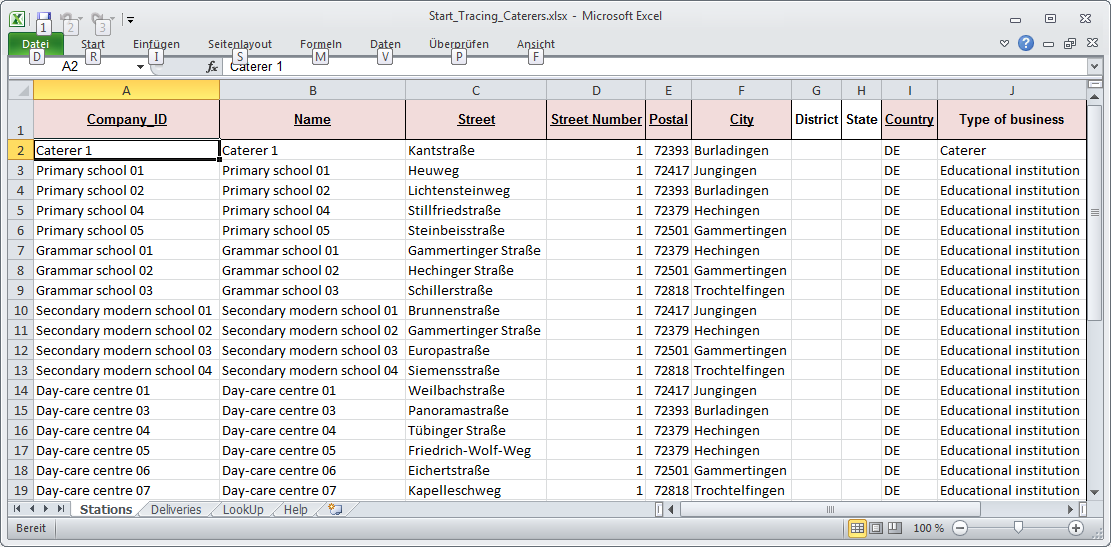
\includegraphics[width=0.95\textwidth]{3.png}
	\end{center}
	\begin{itemize}
		\item For this tutorial we have already pre-prepared a "Start Tracing Template".
		\item Download it from \url{https://github.com/SiLeBAT/BfROpenLabResources/raw/master/GitHubPages/documents/Start_Tracing_Caterers.xlsx}.
		\item In the \textbf{Stations} sheet of this file several \textbf{Educational Institutions} and two \textbf{Caterers} are defined.
	\end{itemize}
\end{frame}

\subsection{4}
\begin{frame}
	\begin{center}
  		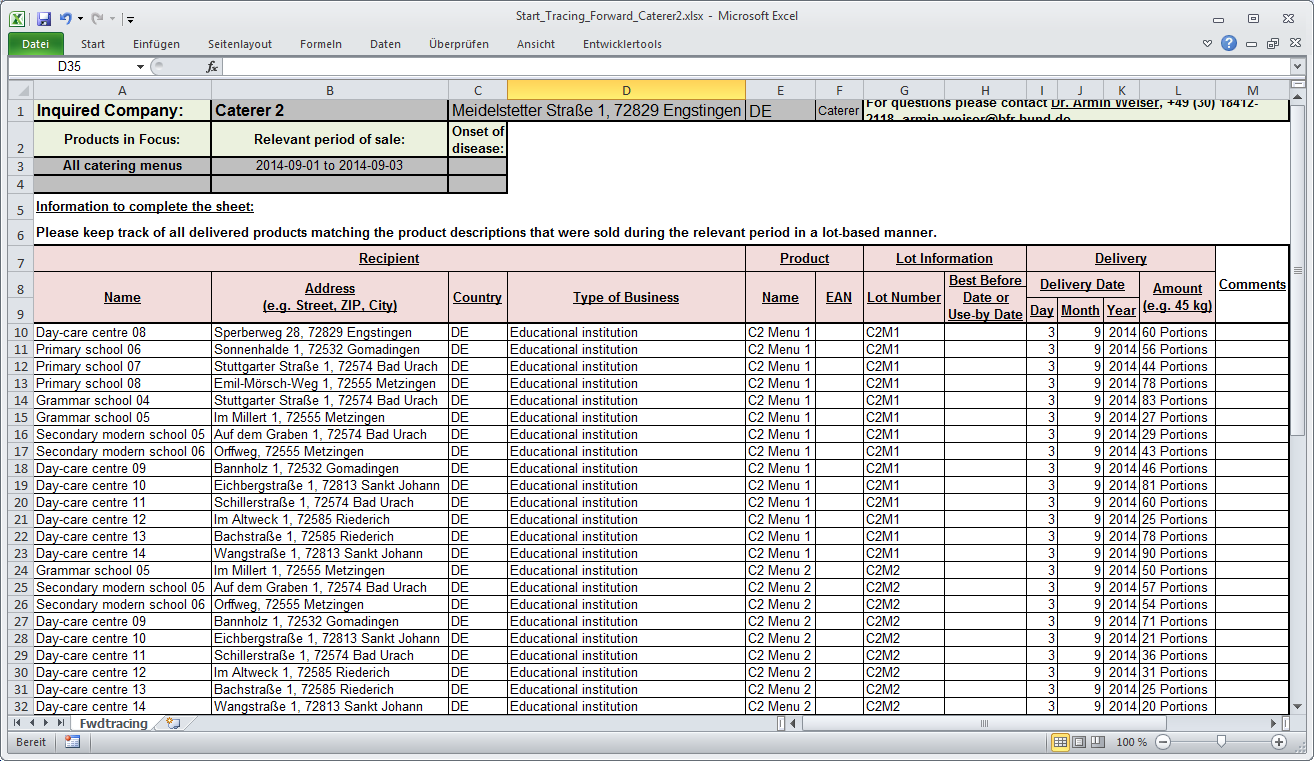
\includegraphics[width=0.95\textwidth]{4.png}
	\end{center}
	\begin{itemize}
		\item Cases of a disease were reported at the \textbf{Educational Institutions}, which received their menus from the \textbf{Caterers}.
		\item The deliveries from the \textbf{Caterers} to the \textbf{Educational Institutions} are defined in the \textbf{Deliveries} sheet.
	\end{itemize}
\end{frame}

\subsection{5}
\begin{frame}
	\begin{center}
  		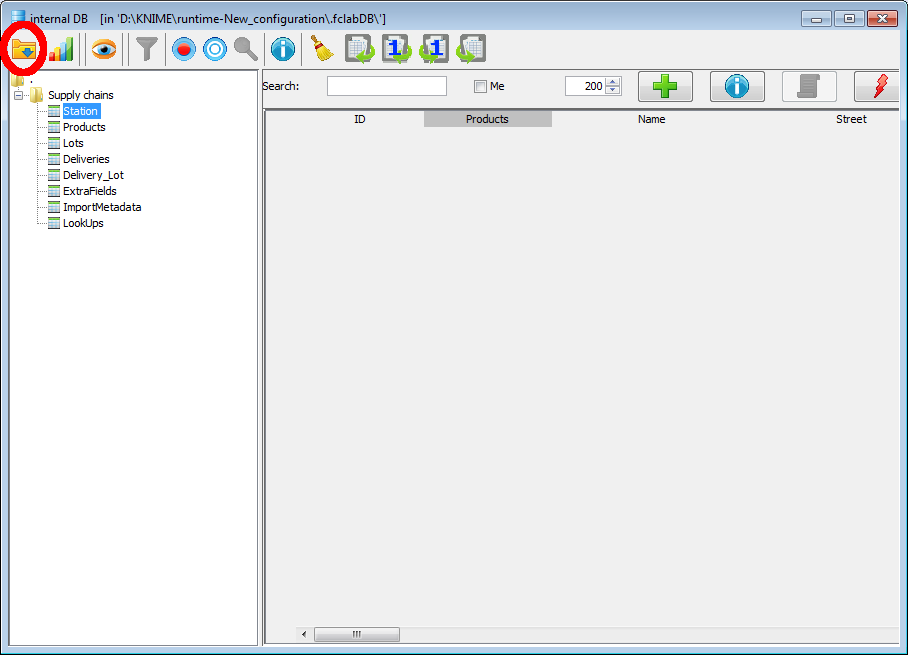
\includegraphics[height=0.6\textheight]{5.png}
	\end{center}
	\begin{itemize}
		\item To import this file click on the \textbf{Table import} button in the upper left corner of the database interface.
	\end{itemize}
\end{frame}

\subsection{6}
\begin{frame}
	\begin{center}
  		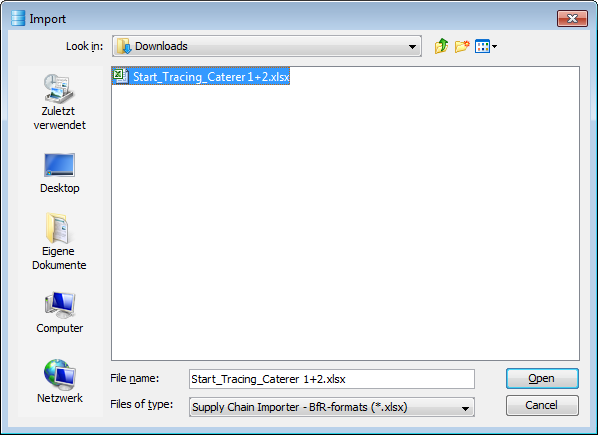
\includegraphics[height=0.5\textheight]{6.png}
	\end{center}
	\begin{itemize}
		\item In the file dialog that appears, select "StartTracing\_Caterers.xlsx" and press \textbf{Open}.
	\end{itemize}
\end{frame}

\subsection{7}
\begin{frame}
	\begin{center}
  		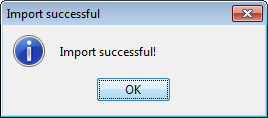
\includegraphics[width=0.4\textwidth]{7.png}
	\end{center}
	\begin{itemize}
		\item You'll see a message that the import was successful.
		\item Press \textbf{OK}.
	\end{itemize}
\end{frame}

\subsection{8}
\begin{frame}
	\begin{center}
  		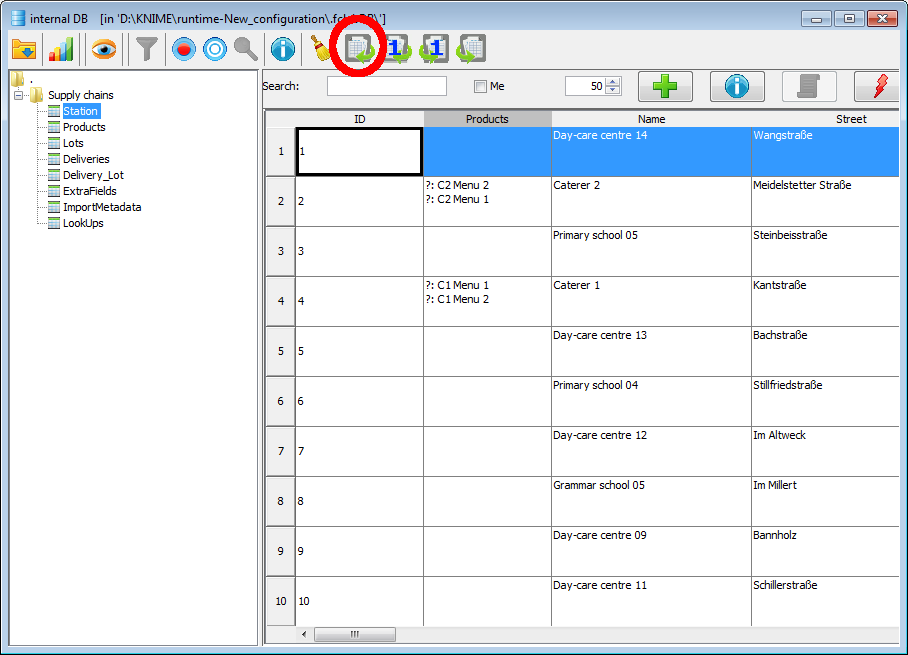
\includegraphics[height=0.5\textheight]{8.png}
	\end{center}
	\begin{itemize}
		\item In the database interface you'll notice, that there is now data in the tables.
		\item Now we want to do a backtracing starting from the caterers to see where they got the ingredient of the meals from.
		\item Press the button for generating backtracing templates, which is marked by the red circle.
	\end{itemize}
\end{frame}

\subsection{9}
\begin{frame}
	\begin{center}
  		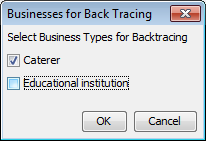
\includegraphics[width=0.4\textwidth]{9.png}
	\end{center}
	\begin{itemize}
		\item Since we want to do the backtracing for the caterers, select \textbf{Caterer} only and press \textbf{OK}.
	\end{itemize}
\end{frame}

\subsection{10}
\begin{frame}
	\begin{center}
  		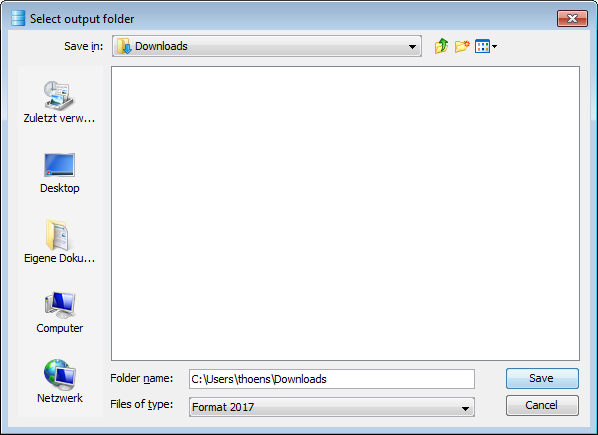
\includegraphics[height=0.5\textheight]{10.png}
	\end{center}
	\begin{itemize}
		\item In the file dialog that appears, you can specify the folder where the generated templates should be saved.
		\item Select or create the desired folder and press \textbf{Save}.
	\end{itemize}
\end{frame}

\subsection{11}
\begin{frame}
	\begin{center}
  		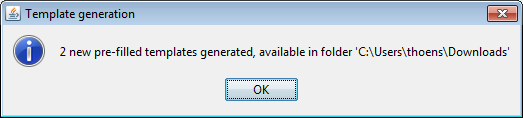
\includegraphics[width=0.8\textwidth]{11.png}
	\end{center}
	\begin{itemize}
		\item You'll be noticed, that 2 templates were generated in the folder you specified.
		\item Press \textbf{OK}.
	\end{itemize}
\end{frame}

\subsection{12}
\begin{frame}
	\begin{center}
  		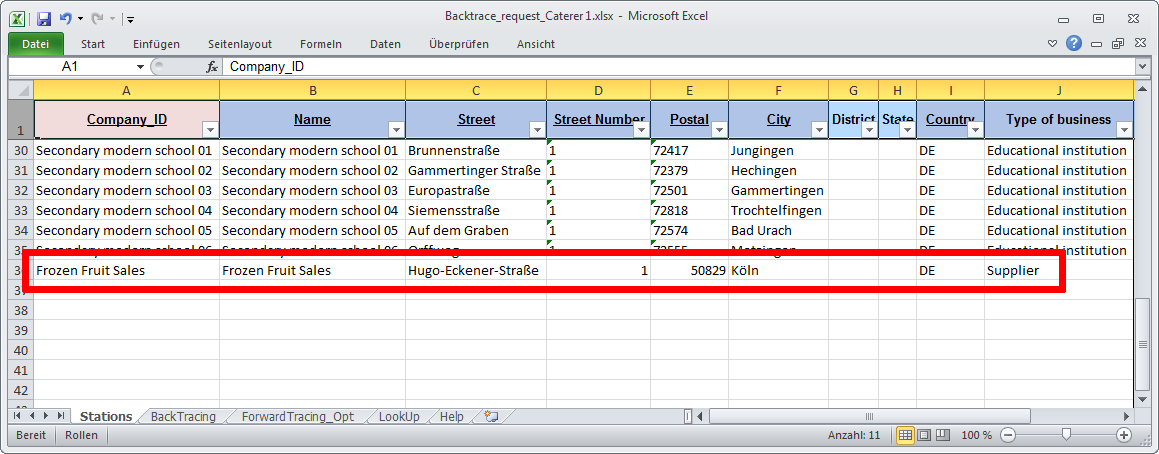
\includegraphics[width=0.95\textwidth]{12.png}
	\end{center}
	\begin{itemize}
		\item To keep this tutorial short, we will only enter the deliveries from one supplier, "Frozen Fruit Sales".
		\item Enter all the information of "Frozen Fruit Sales" in the \textbf{Stations} sheet of "Backtrace\_request\_Caterer 1.xlsx" as you can see in the screenshot.
	\end{itemize}
\end{frame}

\subsection{13}
\begin{frame}
	\begin{center}
  		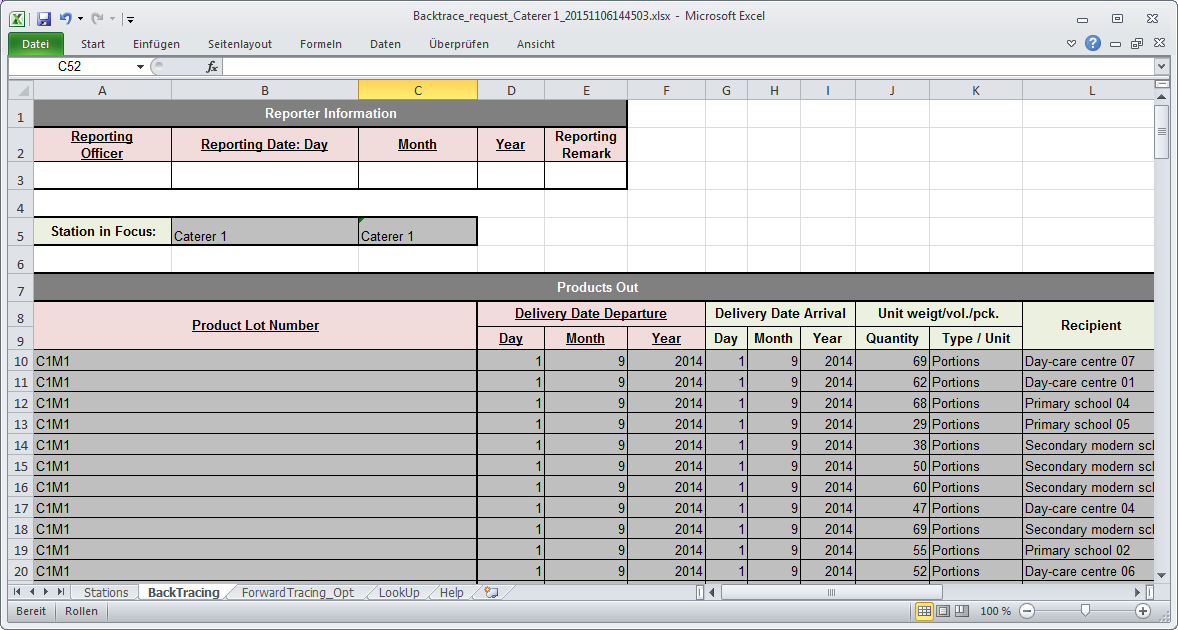
\includegraphics[width=0.95\textwidth]{13.png}
	\end{center}
	\begin{itemize}
		\item Now switch to the \textbf{BackTracing} sheet.
		\item In the \textbf{Products Out} section all deliveries to "Caterer 1" are listed.
		\item These are the deliveries, that we imported from "StartTracing\_Caterers.xlsx".
		\item The deliveries belong to two lots, "C1M1" and "C1M2".
	\end{itemize}
\end{frame}

\subsection{14}
\begin{frame}
	\begin{center}
  		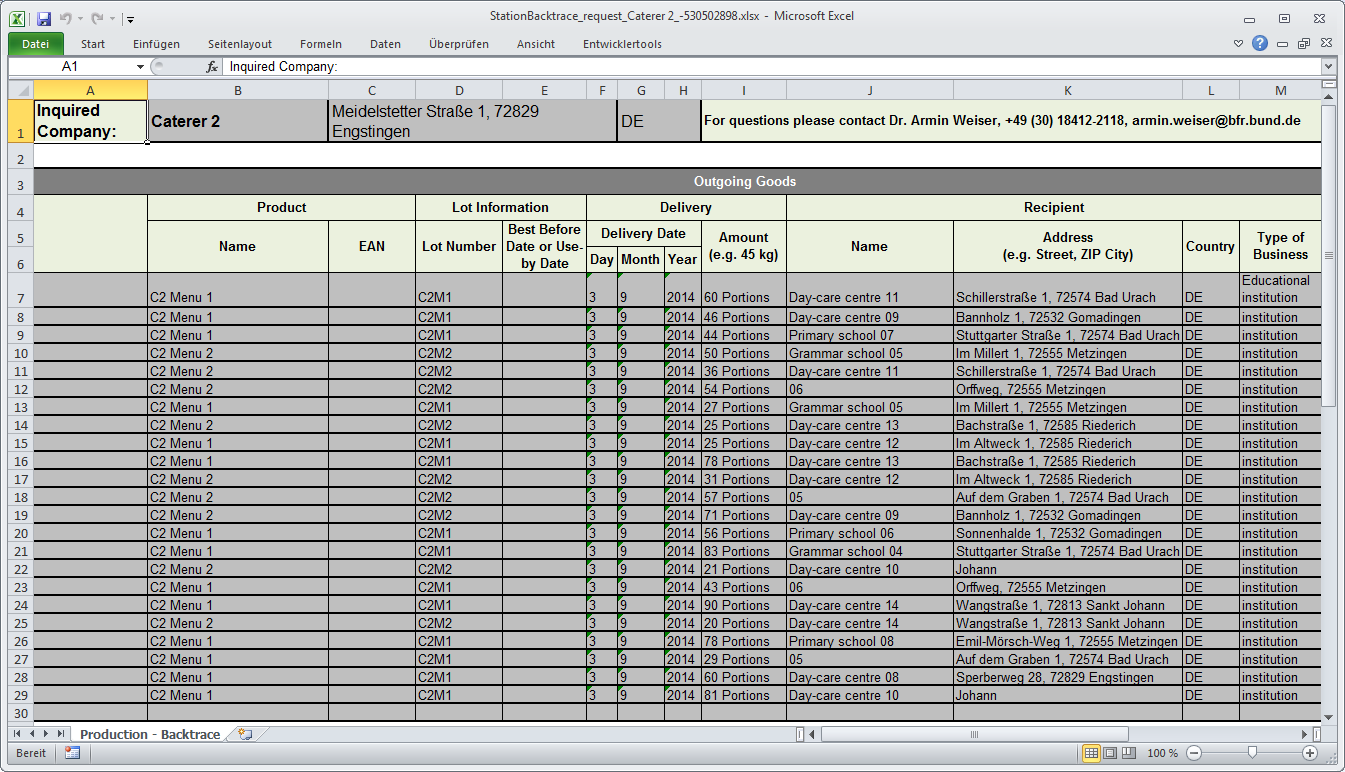
\includegraphics[width=0.95\textwidth]{14.png}
	\end{center}
	\begin{itemize}
		\item Now scroll to the \textbf{Ingredients for Lot(s)} section.
		\item Here you can enter the deliveries received by "Caterer 1" and their associated lots where these deliveries went in as ingredients.
		\item Enter all information for the delivery of "Frozen Strawberries" from "Frozen Fruit Sales" which you can see in the screenshot.
		\item Save the completed document as e.g. "Backtrace\_request\_Caterer 1_completed.xlsx".
	\end{itemize}
\end{frame}

\subsection{15}
\begin{frame}
	\begin{center}
  		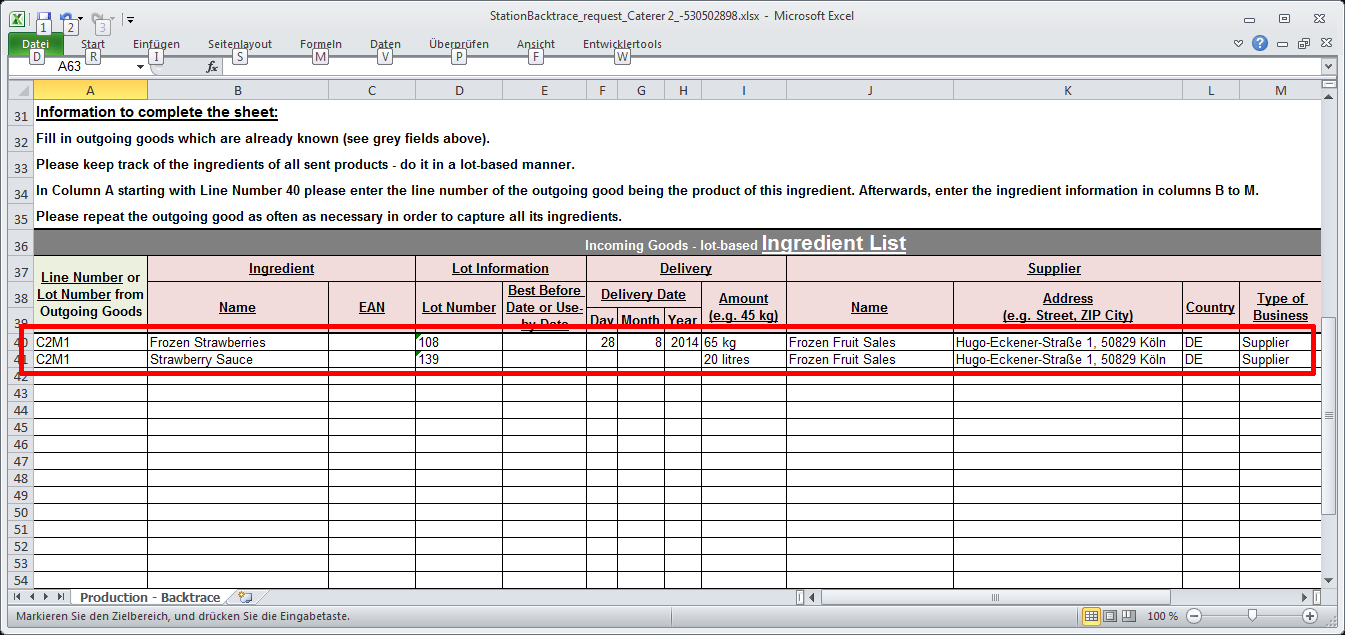
\includegraphics[width=0.95\textwidth]{15.png}
	\end{center}
	\begin{itemize}
		\item Now open the other generated template: "Backtrace\_request\_Caterer 2.xlsx".
		\item Add "Frozen Fruit Sales" to the \textbf{Stations} sheet as we did for the first template.
	\end{itemize}
\end{frame}

\subsection{16}
\begin{frame}
	\begin{center}
  		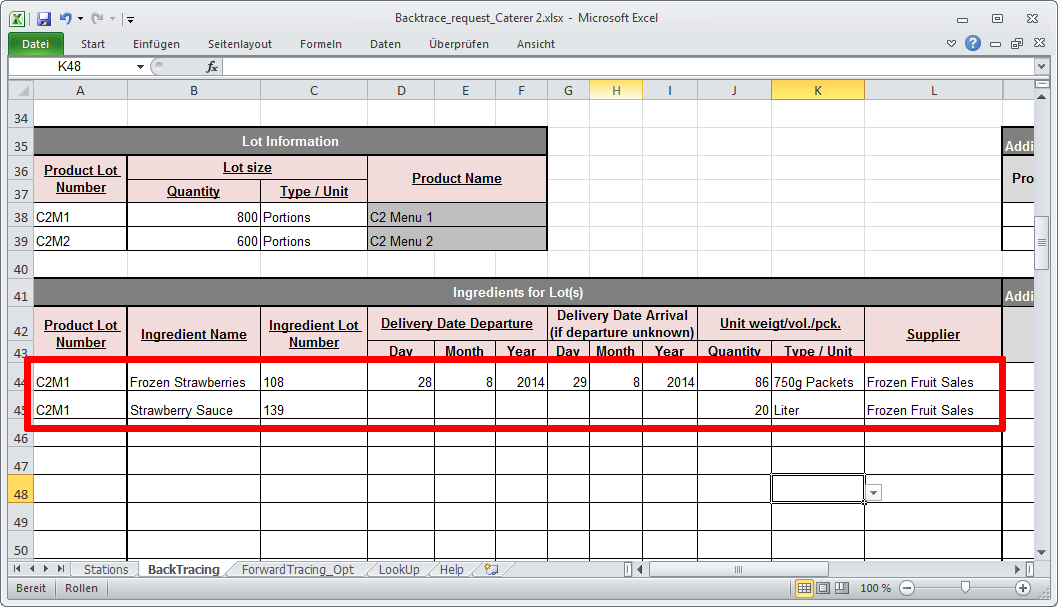
\includegraphics[width=0.95\textwidth]{16.png}
	\end{center}
	\begin{itemize}
		\item Now switch to the \textbf{BackTracing} sheet.
		\item Enter the two deliveries from the screenshot into the \textbf{Ingredients for Lot(s)} section.
		\item Save the completed document as e.g. "Backtrace\_request\_Caterer 2_completed.xlsx".
	\end{itemize}
\end{frame}

\subsection{17}
\begin{frame}
	\begin{center}
  		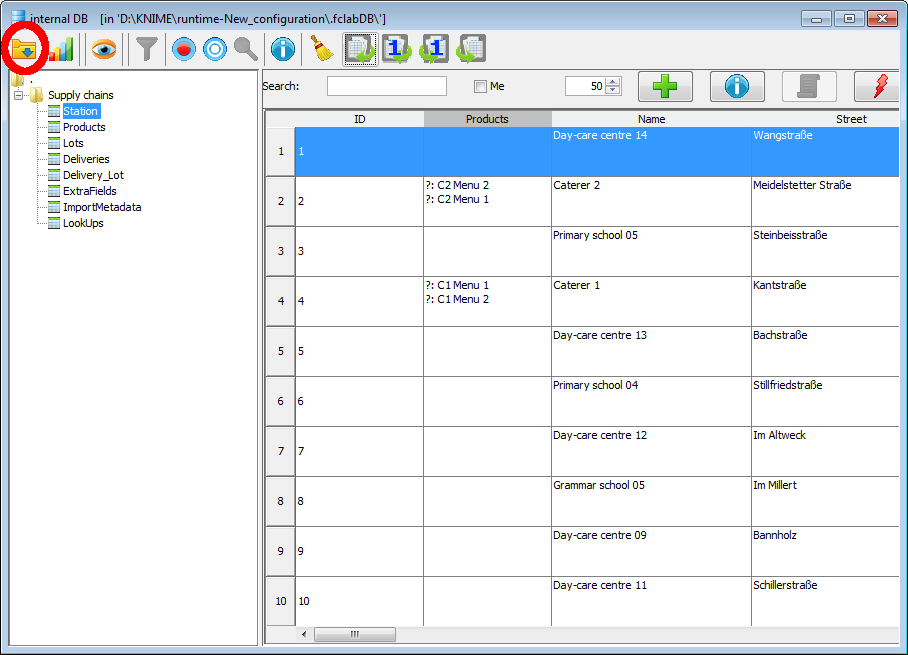
\includegraphics[height=0.6\textheight]{17.png}
	\end{center}
	\begin{itemize}
		\item To import the two files into the database click on the \textbf{Table import} button in the upper left corner of the database interface.
	\end{itemize}
\end{frame}

\subsection{18}
\begin{frame}
	\begin{center}
  		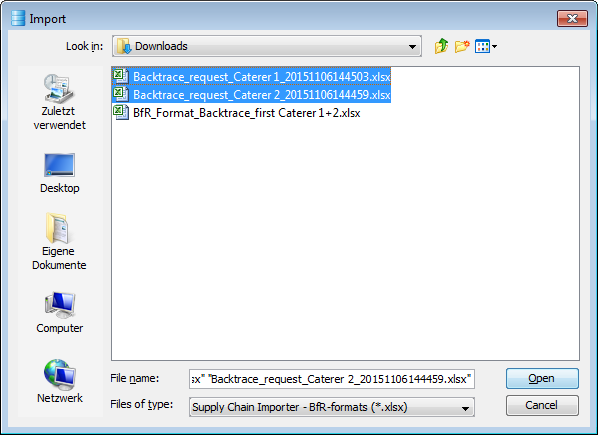
\includegraphics[height=0.5\textheight]{18.png}
	\end{center}
	\begin{itemize}
		\item In the file dialog that appears, select "Backtrace\_request\_Caterer 1_completed.xlsx" and "Backtrace\_request\_Caterer 2_completed.xlsx".
		\item Then press \textbf{Open}.
	\end{itemize}
\end{frame}

\subsection{19}
\begin{frame}
	\begin{center}
  		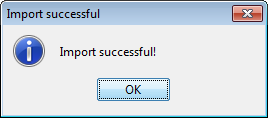
\includegraphics[width=0.4\textwidth]{19.png}
	\end{center}
	\begin{itemize}
		\item You'll see a message that the import was successful.
		\item Press \textbf{OK}.
	\end{itemize}
\end{frame}

\end{document}